% !TEX root = ../thesis-example.tex
%
\chapter{Instances éphémères d'agencements modulaires}
\label{ch:ephemeral}

% \cleanchapterquote{Paradoxalement, la musique du futur est écrite sur du sable!}{Michel Chion}{La musique du futur a-t-elle un avenir?, 1977}

%\cleanchapterquote{Le vieux Paris n'est plus (la forme d'une ville\\
%Change plus vite, hélas ! que le coeur d'un mortel)}{Charles Baudelaire}{Le Cygne, 1861}

\cleanchapterquote{La musique (...) est trop en deça du monde et du désignable pour figurer autre chose que des épures de l'Être, son flux et son reflux, sa croissance, ses éclatements, ses tourbillons.}{Maurice Merleau-Pontry}{L'Œil et l'esprit, 1964} %\cite{merleau-ponty_loeil_1964}

\cleanchapterquote{Dufourt suggests that contemporary music highlights what was rejected in the Greek world : it rather captures the evanescent, the ephemeral, the ambivalent, the Erebus, it favors the endless metamorphosis of qualities and forms; as Nietzsche proclaimed, western music tends toward the liberation of the dyonisiac dimension and the acceptance of the inacceptable part of myths.}{Jean-Claude Risset}{Discours invité à la conférence ICMC, 2014}%\cite{risset_sound_2014} % Remettre cette citation dans le corps du texte.


%\test{blabla}
\section{Paysage des DMIs}
\label{sec:ephemerality:landscape}

%\todo{traduire ce chapitre!}

%--------------------------------------------------------------
\subsection{Les origines}

\subsubsection{Pré-histoire}

Les instruments acoustiques bénéficient d'une histoire vieille de plus de 40000 ans et la finesse de leur fabrication a atteint une excellence qui fait de certains instruments de véritables pièces d'orfèvres. Les instruments numériques sont beaucoup plus récents et ne peuvent rivaliser avec ce degré de raffinement. Pour autant, il ne sont pas totalement déshérités de la tradition et du savoir-faire des instruments acoustiques et par ailleurs, le développement hautement collaboratif à l'œuvre dans le domaine de la programmation informatique fait qu'ils sont, malgré leur jeunesse, des outils extrêmement complexes et les compétences requises pour leur fabrication dépassent souvent de loin ce qu'il serait possible pour un individu seul de concevoir.

Découplage geste et énergie de production dans l'orgue.
Risset dans \cite{genevois_les_1999} ``L'orgue marque le rôle croissant de la technologie dans l'instrument de musique: il introduit le premier interrupteur, le premier clavier, et dès le XVè siècle la première synthèse additive (qui ne sera justifiée mathématiquement par Fouier qu'au XIXè siècle). L'orgue est aussi la première machine informationnelle: l'information donnée par le geste du musicien y est décuplée de l'énergie sonore''\\
Introduction de la mécanique, déport du doigté (Boehm) — révolution industrielle\\
Introduction de l'électricité (théremin, Martenot, patching de la téléphonie)\\
Introduction de l'enregistrement (phonographie, bande, Schaeffer et l'écoute réduite)\\

\subsubsection{L'arrivée du numérique}

1957 : MusicN (Music I en 1957)
1979 : Casio VL-1
1981 : IRCAM 4X
1982 : E-mu Emulator
1983 : MIDI
1983 : DX7
1985 : The Patcher
1989 : FTS/ISPW

%--------------------------------------------------------------
\subsection{Instruments augmentés}
notion d'instrument augmenté discutable (quid traverso=>Boehm ?, quid guitare électrique?) cf. \href{{sec:ephemeral:longevity_stability}}\\
smart instruments (HyVibe, MIND Music Labs)

%--------------------------------------------------------------
\subsection{Interfaces commerciales}
1ère génération MIDI : clavier, sax, guitare MIDI\\
2ème génération MPE :  LinnStrument, Seabord, SoundPlane
Synthés hybrides (Berhinger, Arturia, teenage engineering)
%--------------------------------------------------------------
\subsection{Instruments collectifs}
Laptop orchestras (Plork, Slork, L2Ork, etc.), Méta-Orchestre
Liste de langages : \url{https://github.com/toplap/awesome-livecoding#languages}

%--------------------------------------------------------------
\subsection{DIY DMIs}
Le \gls{DIY}, instruments en kit, arduino, bela, modular, ethersense, etc.

%--------------------------------------------------------------
\subsection{Live Coding}
Instrument = soft, Interface = keyboard
CucK, Tidal, TopLap, \gls{ICLC}

%--------------------------------------------------------------
\subsection{Installations sonores et instruments à la frontière}
installations sur le web (e.g. tentative d'épuisement du bruit blanc)
sonification de données
apps musicales pour smartphones

%--------------------------------------------------------------
\subsection{Musical organics}
Un mot sur la classification de Magnusson.
le terme se traduit difficilement. Organics renvoit à l'idée de l'organologie autant qu'à l'idée d'organicité, i.e. l'organisation d'un être vivant, en particulier à son organisation et sa prolifération rhizomatique.

%%%%%%%%%%%%%%%%%%%%%%%%%%%%%%%%%%%%%%%%%%%%%%%%%%%%%%%%%%%%%%%
\section{Une critique de la longévité}
\label{sec:ephemerality:critique}

\subsection{DMI will survive}

La longévité des \glspl{DMI} est une question complexe qui a été soulevée à plusieurs reprises dans la littérature des \gls{NIME} (et d'autres domaines connexes) et a fait l'objet d'un débat croissant au cours de la dernière décennie \cite{baguyos_contemporary_2014} \cite{morreale_design_2017} \cite{bonardi_preservation_2008}. Les auteurs qui se sont intéressés à cette question ont identifié un certain nombre de causes de cette situation, qu'elles soient techniques, méthodologiques ou sociologiques et ont apporté réflexions et propositions pour y remédier, telles que de nouveaux environnements pour concevoir et évaluer les instruments \cite{jorda_digital_2004} \cite{morreale_design_2017}, une meilleure documentation, de nouvelles méthodes pédagogiques et la création de communautés ainsi qu'un travail visant à établir une notation musicale et un répertoire pour ces nouveaux instruments \cite{mamedes_composing_2014}\cite{mays_notation_2014}. Cependant, dans la majorité de ces articles, le manque de longévité des \glspl{DMI} est essentiellement considéré comme un défaut, ou du moins un problème à résoudre.\\
\indent Dès 1975, des compositeurs de musique électroacoustique au \gls{GRM} réfléchissaient aux questions de préservation soulevées par une musique \iquote{écrite sur du sable}\footnote{Michel Chion utilise cette formule dans \cite{chion_musique_1977}, en faisant référence aux particules ferro-magnétiques des bandes audio, vouées à une dégradation prochaine} : certains compositeurs disaient qu'ils s'en moquaient et faisaient leur musique pour le présent, tandis que d'autres voyaient dans l'ère numérique naissante la possibilité de préserver leurs œuvres dans le futur. Comme nous le savons aujourd'hui, troquer le sable contre le silicium (ou le nuage, maintenant) n'a pas totalement résolu le problème.\\
\indent Les \glspl{DMI} ayant largement intégré la partie compositionnelle des œuvres musicales, parfois même confondue avec l'instrument, le désir de préserver les œuvres musicales s'est trouvé partiellement transposé dans la question de la conservation des instruments et des outils utilisés pour leur production. Mais quelles sont les raisons de cette quête de longévité ? Et qu’est ce qui légitime à ce point la longévité d’un instrument pour qu’elle soit d’emblée vue comme une qualité ? 

\indent Le désir de longévité est lié ontologiquement à une réaction profondément enracinée dans notre condition de simples mortels, qui consiste à chercher un moyen d'assurer notre survie, notamment par la transmission des connaissances et la création de traditions. Le paléoanthroplogue André Leroi-Gourhan a analysé le phénomène des traditions comme un moyen d'extérioriser et de transmettre notre mémoire à travers la création de systèmes techniques et de ``chaînes opératoires'' \cite{leroi-gourhan_geste_1964}. Plus récemment, Bernard Stiegler s'est appuyé sur cette idée (todo : faut il citer aussi Simondon et Auroux ici?) pour définir le concept de ``grammatisation'', comme processus par lequel le continuum temporel des comportements humains est transformé en un spatial discret, ce qui permet de les intégrer dans des outils \cite{stiegler_for_2010}.\\
\indent Les humains ont ainsi développé des méthodes et des outils tels que la psalmodie de textes (surtout religieux), ou l'écriture comme moyens à la fois d'enregistrer des informations pour un usage ultérieur et de transmettre des connaissances à ceux qui y survivent. L'écriture a partiellement libéré l'homme du besoin de tradition orale en transférant ces connaissances sur un support physique, ce qui lui a également permis de capitaliser et de spéculer sur ses connaissances.\\
\indent Ainsi, la notion de longévité traverse le champ des arts et des sciences, aux frontières desquels se trouvent les instruments de musique. Dans l'histoire de l'art, il reste principalement les œuvres durables, ``gravées dans la marbre'' dont sont faites les sculptures. De même, la science aspire à trouver des lois durables pour décrire le monde observable, et les formuler dans le langage pérenne des mathématiques. Mais si la longévité évidente d'une œuvre constitue souvent un atout pour sa propre légitimation, lorsqu'il s'agit d'un instrument numérique, et plus encore lorsqu'il est conçu comme un moyen interactif de créer une expérience musicale par essence éphémère, la question ne semble pas pouvoir se régler dans les mêmes termes.\\

	
\subsection{Longevité, adoption, succès}
Deux aspects semblent être souvent confondus : la longévité d'un instrument d'une part et son ``succès'' d'autre part. De plus, la notion de succès, éminemment sujette à la perspective adoptée, semble être souvent considérée comme le taux d'adoption par une communauté d'instrumentistes, au delà des aspects financier d'un succès commercial.\\
\indent Ces trois aspects, longévité, succès et adoption, sont cependant relativement différents, en partie indépendants et même parfois contradictoires. Il existe des exemples notoires de ce décalage: The Hands de Michel Waisvisz \cite{torre_hands:_2016} (Figure \ref{fig:ephemeral:Waisvisz_TheHands}) ou encore le Méta-Instrument de Serge De Laubier \cite{couprie_meta-instrument:_2018} (Figure \ref{fig:ephemeral:DeLaubier_MI4}) sont deux instruments ayant eu une longévité remarquable\footnote{Plus de 20 ans pour The Hands —jusqu'au décès de Michel Waisvisz, et plus de 30 ans pour le Méta-Instrument dont l'actuelle 4ème version a été finalisée en 2019.}, soutenue par une pratique régulière de leur inventeurs, sans toutefois avoir été adopté par une large communauté d'instrumentistes. Inversement, l'éphémérité d'un outil ne mène pas systématiquement à une absence de popularité \footnote{Considérons ici tous les gadgets éphémères qui, sous l'influence d'une mode et/ou d'une puissante campagne publicitaire, envahissent le marché, ou encore tous les appareils qui deviennent obsolètes lorsqu'un nouvel appareil les remplace, tel que le smartphone qui, outre le remplacement de nos anciens téléphones, a également balayé d'un coup les lecteurs mp3, les GPS, les consoles de jeux portables, les lampes de poche, les montres, etc.} et encore moins à un manque d'intérêt musical pour les performances réalisées avec ces instruments.

%------------------ Figure : Waisvisz — De Laubier ---------------------
\begin{figure}[!htbp]
	\makebox[\linewidth][c]{%
		\begin{subfigure}[b]{.5\textwidth}
			\centering
			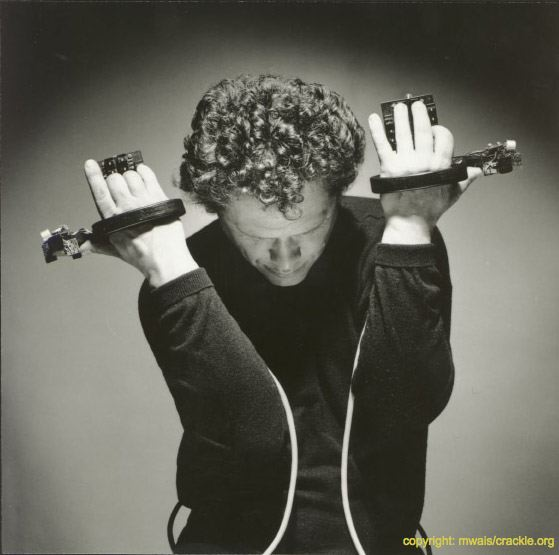
\includegraphics[width=.95\textwidth]{gfx/02_ephemeral/Waisvisz_TheHands.jpg}
			\caption{Michel Waisvisz, The Hands v2\\ photographie: Carla van Thijn}
			\label{fig:ephemeral:Waisvisz_TheHands}
		\end{subfigure}%
		\begin{subfigure}[b]{.5\textwidth}
			\centering
			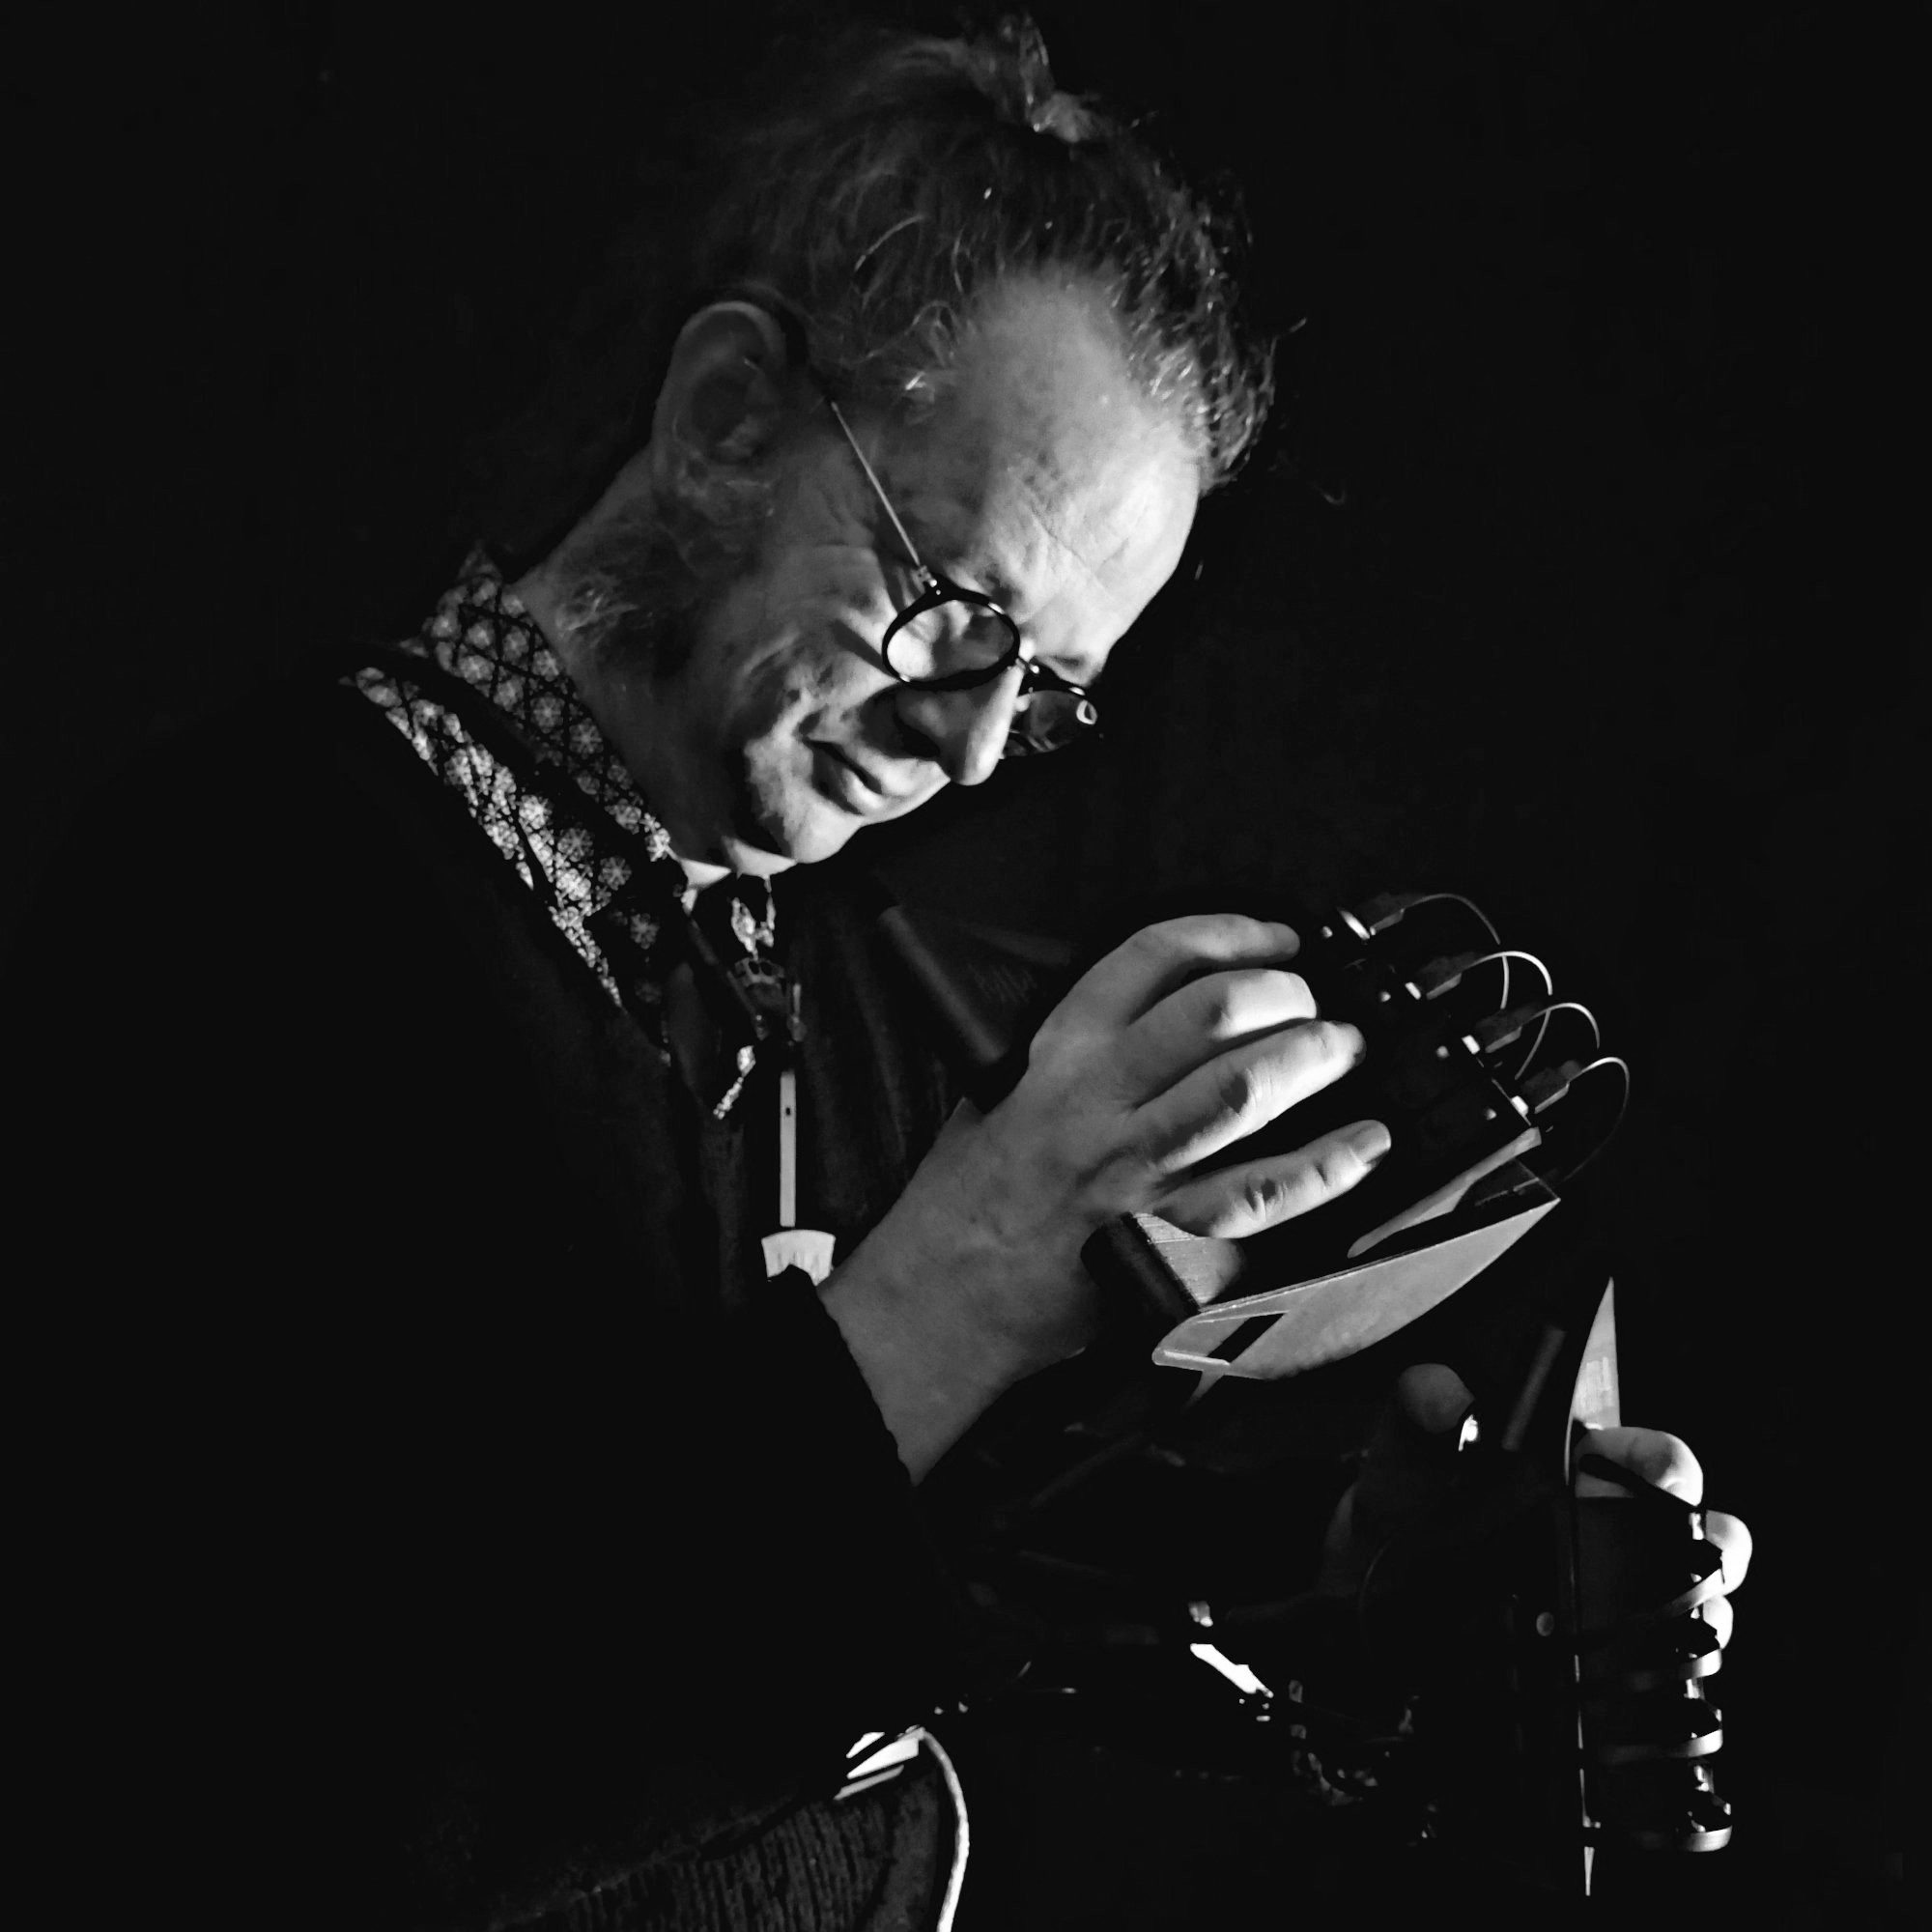
\includegraphics[width=.95\textwidth]{gfx/02_ephemeral/DeLaubier-MI4.jpg}
			\caption{Serge de Laubier, Méta-Instrument 4\\ photographie: Puce Muse}
			\label{fig:ephemeral:DeLaubier_MI4}
		\end{subfigure}%
	}
	\caption{The Hands v2 et le Méta-Instrument 4: durabilité n'est pas synonyme d'adoption}
\end{figure}

\indent La notion de succès dépend ainsi de la perspective adoptée, selon qu'elle soit celle des luthiers qui créent des instruments pour d'autres ou de ceux qui créent des instruments pour eux-mêmes. Dans ce dernier cas, l'adaptation de l'instrument aux besoins ou à l'esthétique propres de l'instrumentiste peut s'avérer telle qu'il soit difficile pour les autres de l'adopter.\\
\indent Egalement, les évolutions techniques ainsi que les modes peuvent amener à la réapparition d'instruments tombés dans l'oubli. On appréciera ici la perspicacité de François-Alexandre Garsault, cité par Malou Haine dans \cite{haine_les_2018}, qui dans sa D``ivision des instruments selon leurs différentes utilisations'' (1761) classait une série d'instruments, dont la harpe et la ``guitare'' (sic), dans la catégorie des \iquote{Instruments hors d'usage, mais qui peuvent revenir.}


\subsection{Longevité versus stabilité}
\label{sec:ephemeral:longevity_stability}
La question de la durabilité d'un instrument soulève implicitement la question de sa stabilité historique. Ainsi, l'histoire organologique des instruments de musique européens révèle de nombreux facteurs qui conduisent à l'apparition, à l'évolution ou à la disparition des instruments de musique. A cet égard, les nombreuses innovations technologiques de la révolution industrielle s'avèrent intéressantes car cette période bien documentée illustre les débuts des grandes révolutions qui allaient se produire au XXe siècle, tout en soulevant la question même de la stabilité de la forme des instruments. Ainsi, lorsque le traverso fut équipée du système de clétage inventé par Théobald Boehm en 1832 et devint une flûte traversière, s'agissait-il d'un nouvel instrument ? À quel moment décidons-nous qu'un instrument qui subit des changements n'est plus le même ?

\subsection{Éphémérité dans le contexte musical}
\label{sec:ephemeral:ephemerality_in_musical_context}

\subsubsection{Impermanence du phénomène sonore}
\noindent Rappelons tout d'abord une évidence : la musique elle-même est intrinsèquement intangible, évanescente et nécessite une énergie entretenue pour exister : le phénomène sonore est en éphémèrité permanente. La musique, dans sa forme sensible, n'existe que pendant le temps de son performance. Bien que les instruments utilisés pour la produire puissent être durables, leur convocation et le son lui-même sont toujours temporaires\footnote{à tel point que les pièces qui mettent au défi cette éphémérité, telles que les Vexations d'Erik Satie ou encore Organ²/ASLSP de John Cage sont des exceptions notoires.}.

\subsubsection{De la performance}

\noindent Même lorsqu'elle est notée sur une partition, la musique en tant que qu'art vivant est en constante réinterprétation. Cette interprétation permet de transformer une partition notée sous forme symbolique en une expression sensible sujette à variations. On peut objecter que cette interprétation n'existe que lorsque la musique est notée de manière symbolique, laissant aux interprètes la possibilité de la jouer à leur façon dans le contexte de l'interprétation. Mais est-ce toujours le cas lorsque la musique est `intégralement notée' jusqu'au son lui-même, comme c'est le cas sur un disque audio ? Cela signifie-t-il que l'interprétation disparaît ? Les performances de spatialisation en direct de la musique électroacoustique par des musiciens professionnels ou les différentes pratiques de remixes que l'on retrouve dans le hip-hop tendent à prouver le contraire. Toute performance musicale, même la simple écoute d'un disque, convoque inévitablement un nouveau contexte d'écoute, car elle se produit nécessairement dans un moment présent unique. Entre le son enregistré et son écoute, on retrouve la même \textit{différance}\footnote{La \textit{Différance} est un concept proposé par Derrida \cite{derrida_lecriture_2014} pour désigner à la fois l'ajournement (le fait de différer) et la différenciation qui se créé entre un texte et sa signification.} qu'entre une partition et ses interprétations.

\subsubsection{Une esthétique musicale mûe par le mouvement}

Par ailleurs, la musique contemporaine occidentale poursuit une quête de la nouveauté et de territoires sonores inexplorés, comme le soulignait Jean-Claude Risset dans son discours à Athènes en 2014 \cite{risset_sound_2014}: \iquote{Dufourt suggests that contemporary music highlights what was rejected in the Greek world : it rather captures the evanescent, the ephemeral, the ambivalent, the Erebus, it favors the endless metamorphosis of qualities and forms; as Nietzsche proclaimed, western music tends toward the liberation of the dyonisiac dimension and the acceptance of the inacceptable part of myths.}

\subsubsection{Partitions dynamiques, ouvertes, ad-hoc}

\noindent Les partitions musicales sont en partie intégrées dans les \glspl{DMI}, pour lesquels Norbert Schnell et Marc Battier ont proposé le terme `d'instruments composés' dans \cite{schnell_introducing_2002}\footnote{L'idée d'instruments composés est toutefois plus ancienne, voir Harry Partch ou Gordon Mumma (1967) : \iquote{I consider that my designing and building circuits is really ‘composing’ y my ‘instruments’ are inseparable from the compositions themselves.}\cite{mumma_creative_1967}}. La partition elle-même a fait l'objet d'une reconfiguration plus ouverte depuis le milieu du XXe siècle et les compositeurs ont progressivement intégré les possibilités algorithmiques dans leurs processus de création : des systèmes dynamiques et interactifs mettent en mouvement la stabilité des figures de notes. Plusieurs compositeurs\footnote{Parmi ceux qui ont écrit et analysé des partitions dynamiques, voir les œuvres de Hajdu \cite{hajdu_disdisposable_2016}, Bhagwati \cite{bhagwati_vexations_2017} ou Freeman \cite{freeman_extreme_2008}} questionnent ainsi la stabilité de la partition en utilisant l'ordinateur pour créer des instances \textit{ad hoc}, soit à l'aide d'algorithmes génératifs, soit en introduisant des parties improvisées dans des formes hybrides pour lesquelles Richard Dudas propose le terme de ``comprovisation'' \cite{dudas_comprovisation:_2010}. En est-il ainsi, que la technologie numérique offre ce support idéal qui permettrait à la fois la préservation des œuvres musicales en même temps que leur mutation ?

\subsubsection{Obsolescence de la technologie}

The materials used for acoustic instruments seem to age relatively well. Electronic hardware ages poorly in comparison, and the copper of its circuits is more fragile than that of brass instruments. Moreover, the extreme miniaturization of microprocessors often makes them impossible to repair; they need to be replaced and there is great chance that the substitutes will be new, different versions. Computer code, in its compiled form, is just as cryptic as the microprocessor: an unreadable block that embodies the paradox of computer-based notation as compared to traditional paper—we are writing things which we can no longer read. And when the operating system is updated, chances are it will no longer be able to read them either.\\
In an article where he compares the ontological differences between hardware and software, Nicolas Collins \cite{collins_semiconducting_2013} summarizes their relation to time with the formula: \iquote{hardware is yesterday, software is now}, what could be translated as the fact that software is under permanent update while hardware is ever outdated. Neither seems to be able to offer a reliable continuity between the past and the future.


	
\subsubsection{Economie de la nouveauté}

In addition to the obsolescence of technology, DMIs are confronted with the effects of consumer society. For more than a century, the industry has increasingly promoted a disposable paradigm by encouraging consumers \iquote{to trade for style, not just for technological improvements} \cite{slade_made_2006} and while organizing planned obsolescence.\\
\indent This economic model also affected that of the performing arts, which promotes creations much more than the revival of a show to such an extent that, as Georg Hajdu recalls in \cite{hajdu_disposable_2016}: \iquote{Pieces rarely see more than a single performance} Artist residencies are likewise targeted towards new creations and rarely propose the continuation of previous works.\\
\indent This economy of obsolescence (planned or not) does not favour attachment to an instrument and, as far as commercial MIDI controllers are concerned, the cheap plastic they are most often made of degrades the value that can be attributed to a traditional acoustic instrument. The attachment and commitment to a virtual instrument is also challenged by its virtual nature. Most commercial software is now moving towards a rental—rather than purchase—economy, since the purchase no longer guarantees the sustainability of the property.
	
\subsubsection{L'instrument comme compromis instable}

The musical instrument is also, as Bernard Sève points out in \cite{seve_instrument_2013}: \iquote{an unstable compromise between non-convergent qualities}. For acoustic instruments, this compromise between gestural ergonomics and acoustic performance, imposed by the physicality of the materials, is generally fixed in a fitted and glued assembly. This bonding acts as a stabilizing factor compared to a digital environment in which the absence of physical constraint leaves the instrument open-hearted, ready to be modified at any time.\\
\indent Bill Buxton pointed out the difference between standard, military and artistic specifications to underline the higher requirement of the latter \cite{buxton_artists_1997}. Art-driven design require great finesse indeed. Tuning the sonic and ergodynamic\footnote{Magnusson proposed this term in \cite{magnusson_ergodynamics_2019} to name the \iquote{expressive power and depth of an instrument}.} qualities of a musical instrument is a quest for an inframince\footnote{Marcel Duchamp \cite{duchamp_notes_2008} coined the term inframince in a series of examples depicting a difference so small that it can only be imagined.} for which there is no agreed specifications. But another particularity of the technologies used for live performance is that they are \iquote{devoted to an experience, not a sound track; unavailable for reshuffle or back-up or exchange or duplication}, as Nicolas Collins notes in \cite{collins_semiconducting_2013}.\\
\indent Thus, the sustainability of the instrument outside the very duration of performance is not an essential criterion and it is not uncommon for digital musicians\footnote{Andrew Hugill defines a \textit{digital musician} in \cite{hugill_digital_2019} as \iquote{one who has embraced the possibilities opened up by news technologies, in particular the potential of the computer for exploring, storing, manipulating and processing sound, and the development of numerous other digital tools and devices which enable musical invention and discovery} underlying the fact that they are \iquote{not defined by their use of technology alone}, but also have \iquote{a certain curiosity, a questioning and critical engagement that goes with the territory} .} to modify their instrument minutes before the beginning of a concert, just for the needs of the present moment.
	
\subsubsection{Esthétique du dysfonctionnement}

Indeed, the risk of dysfunction is not a major obstacle to many musical performances. Bugs and artefacts caused by malfunctions are proving to be fertile sources of musical materials and subverting the cryptic functioning of processors reveals an invisible aspect of them, bringing to the surface their very nature, beyond the purpose for which they were designed\footnote{Among significant examples, Yasuano Tone's works on “wounded CDs”, Nicolas Collins's works on dead circuitry or Carsten Nicolai's sonification of raw data exemplifies this approach.}. David Zicarelli, quoted by Cascone in \cite{cascone_aesthetics_2000}, sums it up in these terms: \iquote{I would only observe that in most high-profile gigs, failure tends to be far more interesting to the audience than success}.

\subsubsection{Plus besoin de tradition?}

The appearance of musical notation made performance no longer necessary for the only purpose of transmission; audio recording made performance no longer necessary for the only purpose of listening; computers and sound banks made the learning of a particular instrument no longer necessary to produce the sound of that instrument\footnote{See for example, the rendition of Stravinsky's Rite of Spring by Jay Bacal with VSL. https://youtu.be/PB3njyDW8SY.}; and now, artificial intelligence makes the very act of composing no longer necessary for music to be composed\footnote{See for example the outcomes of the FlowMachines project by François Pachet et al. in \cite{hadjeres_deepbach:_2016}: “Daddy's car” (\url{https://youtu.be/LSHZ_b05W7o}) or “DeepBach” (\url{https://youtu.be/QiBM7-5hA6o}).}.\\
\indent In 1964, Leroi-Gourhan, who saw in the computing machine the unprecedented possibility of outsourcing memory, was wondering what would happen if the machines became capable of \iquote{writing perfect plays, creating inimitable paintings} \cite{leroi-gourhan_geste_1964}. In 1992, John Cage seemed to answer him a radical way, when saying: \iquote{We don't have to have traditions if we free ourselves from memory} \cite{sebestik_ecoute_1992}. \\
\indent However, if it is possible to evolve, as Buci-Glucksmann describes it in \cite{buci-glucksmann_esthetique_2003}, from a culture of the object to a culture of flows, she remarks that in a country like Japan that values impermanence positively, the ephemeral has a central place while being deeply rooted in tradition.	\\
\indent The resolution of this apparent antagonism between Cage's position and Buci-Glucksman's seems to lie in the displacement of objects (or flows, for that matter) supported by tradition, in the reformulation of the motivations for sustainability and ephemerality.


\section{Articulation du pérenne et de l'éphémère}

\subsection{Les DMI comme agencements instables et sauvages}

The very term DMI, which has gradually invaded the NIME literature, may lead us to believe that it is a well-defined category when it is in fact a hodgepodge of objects only sharing their use of digital computation. A resulting bias in the assessment of the failure of DMIs to reach maturity stems from the fact that a musical instrument is often still considered as a coherent whole, requiring longevity, similar to the acoustic instruments taken as role models.\\
\indent Yet, the modularity induced by electronics and digital technology has atomised the integrity of the instrument. This atomisation can both be understood in the sense of “destructed” but also in the sense of “fragmented into atomic bits”. On stage, we can further observe that DMIs are often fragile (cf. Figure \ref{fig:ephemeral:Gordeff}), prototypical assemblies, full of cables ready to be interchanged minutes before the concert, or even during it. So why should we consider DMIs as durable monoliths rather than ephemeral assemblages\footnote{Following Deleuze and Guattari's concept proposed in \cite{deleuze_mille_1980} voir aussi ``musical instruments as assemblage'' de Paul Theberge.} that they most often are?\\
\todo{évoquer la notion de behavioural objects de \cite{bown_understanding_2009}}
\indent From this point of view, the academic format of a conference such as NIME makes it difficult to present DMIs in their chaotic form and their selection is biased by the fact that their authors often belong to the academic world. This favours a demonstration of duly considered technical criteria rather than the presentation of a chaos of hectically connected algorithms whose functioning is not really understood, except for the fact that the musician who plays them does wonders.\\
\indent By confronting an ephemeral instrumental setup, the instrumentalist, however virtuosic they may be, necessarily finds themselves in tension with a wild instrument to tame. This calls for an intense gestural and auditory attention and the research of resonance with the instrument. (Otherwise, one might as well compose comfortably at home and provide the listener with an audio record to be played with a single button). Maybe more important than longevity, here is an interesting design criterion for digital lutherie: the possibility that the instrument spins out of control.

%-------------------------- Figure : Gordeff ----------------------------------
\begin{figure}[!htbp]
	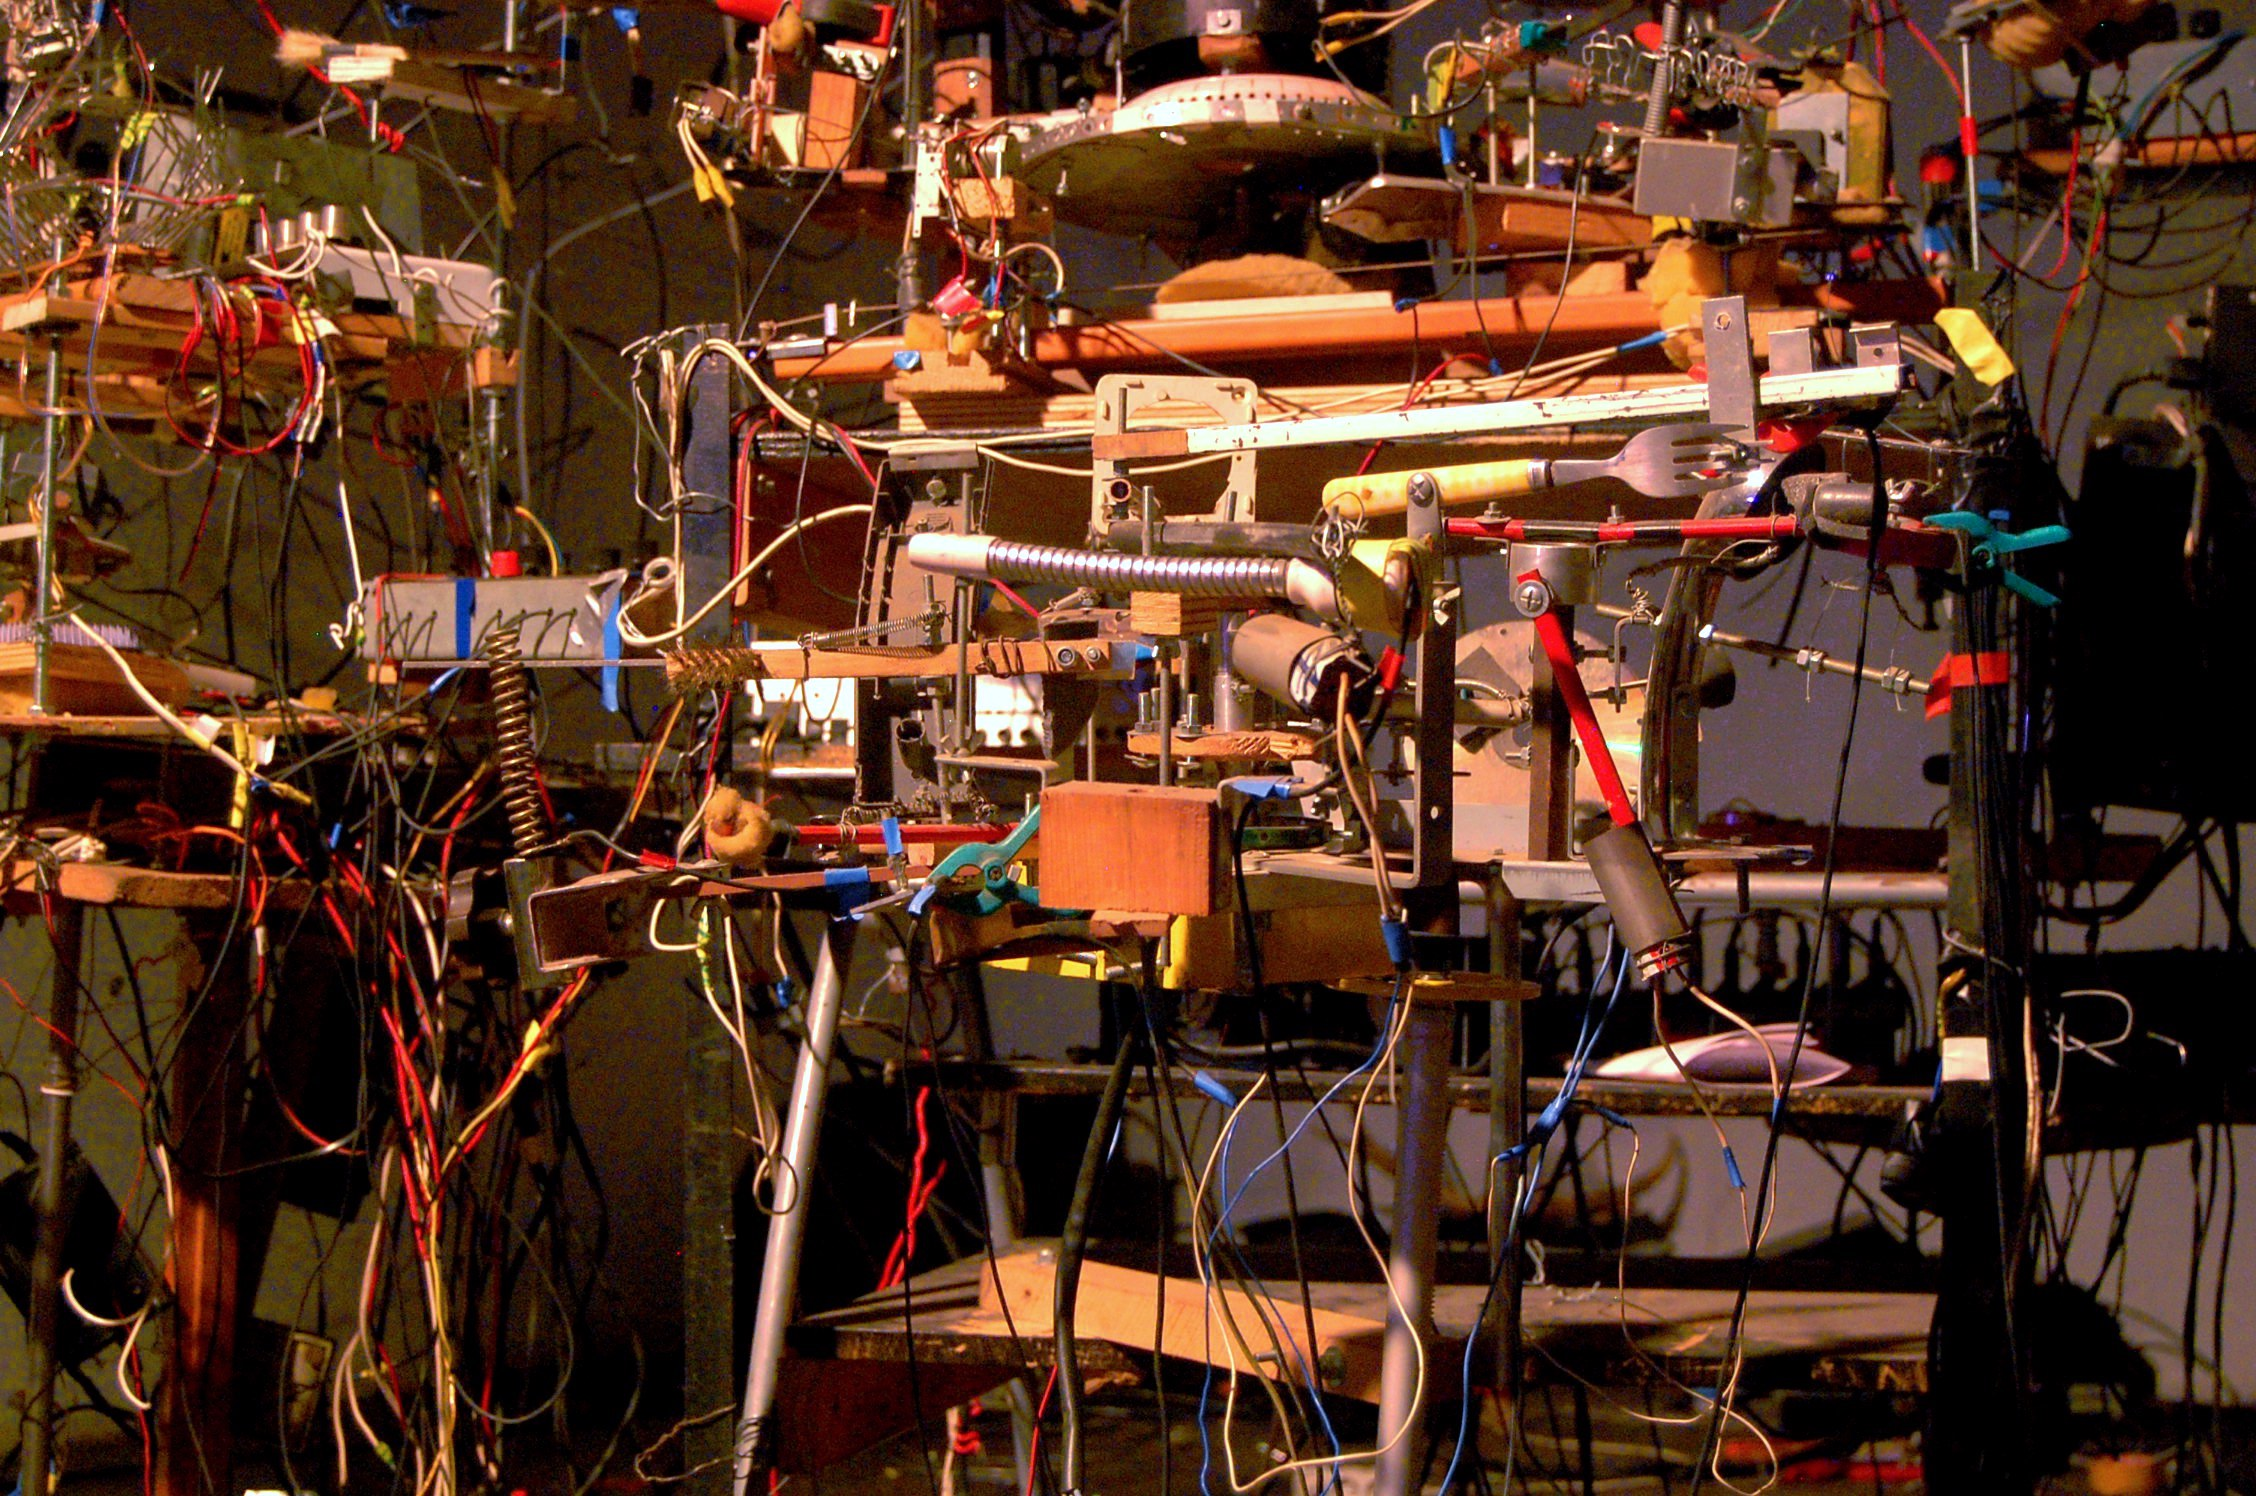
\includegraphics[width=\textwidth]{gfx/02_ephemeral/PierreGordeff.jpg}
	\caption{Détail d'un instrument de Pierre Gordeff.}
	\label{fig:ephemeral:Gordeff}
\end{figure}

\todo{rajouter une réf et un mot sur Fragile Instruments \cite{haddad_fragile_2017}}

\subsection{Cuisiner des instruments à la volée}

Another reason that contributes to the stability of acoustic instruments is related to their physicality and manufacture, which requires a considerable amount of work compared to the virtual arrangement of software blocks—it takes more than two months to build a cello for a luthier who knows his job! Conversely, Bowers and al. promoted the use of readymade objects as half-made infra-instruments \cite{bowers_not_2005} and “pin-and-play” ad-hoc instruments \cite{bowers_creating_2006}, while rethinking the life-cycle of an instrument with such kind of quickly-built ephemeral assemblages.\\
\indent More generally, as one create a DMI with an audio programming environment, the software not only provides basic functions but comes with libraries, ready-made examples, supplemented by countless online resources, ready to be downloaded, copied and pasted.\\
\indent This means that the building of a DMI can be a much faster subtractive process: rather than starting from a blank page, it is possible to search for a version close to what one wants to achieve and modify it from there. Nicolas Collins compared this simplicity to cooking, emphasising its democratisation: \iquote{What it means is that if you are doing live performance, if you do need specialized instruments, it's almost more like cooking than it is building musical instruments. Everybody cooks, you don't need to go to ‘chef schools’!} [Collins, personal communication TODO = annexe].\\
\indent Recent evolutions in audio-programming languages tend to address the issue of sustainability by creating Domain Specific Languages that can be exported to various targets. Hardware platforms like Bela or The Owl\footnote{Bela: \url{https://bela.io}; The Owl: \url{https://www.rebeltech.org}} and languages like FAUST \cite{orlarey_faust_2008} or the announced SOUL language by Roli\footnote{Announced at the Audio Developer Conference 2018. \url{https://youtu.be/-GhleKNaPdk}} all reflect this trend. It is worth noting that FAUST, which was designed with preservation in mind\footnote{FAUST was a key component of ASTREE, a project focusing on the preservation of musical work with electronics.}, actually helps building ephemeral instances by offering both an online compiler and just-in-time compilation.
	
\subsection{Une relation tri-partite : répertoire / musicien / contexte}

If we therefore stop considering the ephemerality of instruments as a problem, we can consider how longevity and ephemerality can be articulated in the agency of DMI practices. It can be conceived as a tripartite coupling between materials, musician and context. Each component of this triad may then has a different degree of stability.

\subsubsection{Le grand répertoire}

The components of a DMI can be considered as belonging to a large repertoire of both material and immaterial heritage. The material repertoire includes any physical material that can be used in the construction of acoustic instruments: raw materials as well as manufactured, machined or mechanical parts. \\
\indent The immaterial repertoire is all the theoretical knowledge and cultural heritage one can rely on during the making of an instrument\footnote{Obviously, practical knowledge is also essential to the making of an instrument, although it does not really belong to the shareable heritage to which I refer here.}: music theory, scientific and technical knowledge, established playing techniques, musical repertoire, etc. This knowledge helps to shape the materials and imprint musical markers to create the instrument: the placement of frets, the tuning of strings, the layout of keys, etc.\\
\indent In the case of DMIs however, the repertoire of physical materials is considerably expanded by reified knowledge available as digital materials, either in the form of computer code or datasets (e.g. audio samples, impulse responses, scores, etc.) that enables the musical qualities of an instrument to to be shaped beyond what is possible with physical materials.
This set, as heterogeneous as it may seem, constitutes a shareable repertoire from which digital luthiers can draw the necessary ingredients for the design of their instrument.

\subsubsection{Le musicien in-progress/in-process}

The second element of the assemblage is the musician\footnote{Here the generic term “musician” mainly represent the instrumentalist the blurring roles of instrumentalists, composers and luthiers. The instrumentalist is not necessarily present during the performance—the instrument can be autonomous, but their presence is then implicit as a luthier or composer, the boundaries between these roles have been largely blurred since the 20th century.}. Musicians are alive and subject to change: their knowledge, feelings and desires, musical skills and awareness, projects and physical capacities, all evolve during their existence. This evolution is reflected in the instrumental device, by the addition or removal of features, or the development of new instruments related to a new musical project. Just like you may learn to ride with a bicycle equipped with side wheels and later remove them, DMI can offer evolutive assistance for progressive learning. A co-dynamic relation with one's instrument can help improve the intimacy between the musician and the technical object becoming an instrument.

\subsubsection{Le \textit{hic et nunc} de la performance}

Eventually, the DMI can be adapted to the context of performance, which is generally more ephemeral than the two aspects mentioned above.\\
\indent Expanding their own musical repertoire by drawing on the grand repertoire mentioned above and on their own experience, musicians selects a subset of elements in the perspective of a particular performance, for a singular artistic proposition, and to meet the spatial and temporal conditions of the performance, as well as the audience. As an example, the costless duplication of code offers possibilities to rescale DMIs from soloist to collective instruments by distributing control over multiple interfaces. New projects can imply starting from scratch, but existing ones often only involve contextual adjustments rather than a thorough reprogramming of one's system. Kiefer and Magnusson coined the term “pre-gramming” \cite{kiefer_live_2019} to describe that particular kind of preparation.
	

\section{Jouer d'un DMI éphémère}

As we can see, creating a DMI can be a very fast process as it can be done by simply assembling already pre-built elements. But once the assemblage is done, how do we learn to play it?

\subsection{Composition, conception, apprentissage et jeu en parallèle}

\indent Traditional acoustic instruments are supported by methods and repertoire that can rely in turn on the instrument's stability. But for a new—possibly unique, possibly ephemeral—DMI, such resources are scarcely available. Software comes at best with manuals, but manuals usually explain how to make the software run, not how to play music with it.\\
\indent From there, the learning process can follow two seemingly opposite directions: finding the right moves to play desired sounds and finding the right sounds for chosen gestures. A consequence is that often, learning a new DMI starts right from its conception and is a co-dynamic process that accompanies its development up to the \textit{pre-gramming} of the instrument, with back and forth between moments of play and moments of adjustment.

\subsection{Entrer dans l'avenir à reculons}

DMIs and their practices integrate the know-how inherited from electroacoustic music since the middle of the 20th century. The pedagogy of electroacoustic music essentially developed a musical theory of listening \cite{schaeffer_traite_1966} and metaphors for composing \cite{bayle_musique_1993} but conceived at a time when electroacoustic music could only be composed, before real-time audio allowed live practices. As a result, these theories were more oriented towards musical composition than performance as such.\\
\indent In the absence of established musical notation for sound, experimental electronic music is largely oriented towards free improvisation. This implies a letting go enabling the instrument to express its potentialities and a practice of “aurality”\footnote{Described by Alain Savouret as a music theory for the audible.} to “enter the future backwards” \cite{savouret_introduction_2010} and react to what is coming out of the instrument rather than completely controlling it.
	
	
\subsection{Trouver les résonances}

The learning of an instrument (beyond the learning of the heritage idioms of this instrument) thus requires a search for resonance. We can experience this resonance at an acoustic level, but more generally as an empathetic resonance, which consists in immersing ourselves in the instrument to find the spaces that will (re)sound satisfactorily, to find the “sweet spots” where what we hear meets what we were seeking—sometimes unknowingly. Since mathematical linearity is rarely satisfactory at a perceptual level, this exploration involving the coordination between play and critical listening is essential to adjust the mapping functions that will define the instrument's behaviour.
	
\subsection{Entomologie musicale (bestiaire)}
The musical exploration of a DMI brings out unknown musical forms, like ephemeral butterflies. Learning a DMI therefore often involve an entomologist-like task of pinning these sonic creatures and giving them a name. This naming will allow to come back to them later on (by saving them in presets for example) as well as to discuss with other musicians about a performance which, in the absence of established musical idioms on which to rely—like scales or time signature— can be cruelly lacking references. Such a task was led in the development of “John, the semi-conductor”, an open score system described in \cite{goudard_john_2018} (TODO : renvoyer au chapitre notation).\todo{fusionner avec la section \ref{sec:ephemeral:vessels}?}



%-------------------------- Figure : Entomologie ----------------------------------
\begin{figure}[!htbp]
	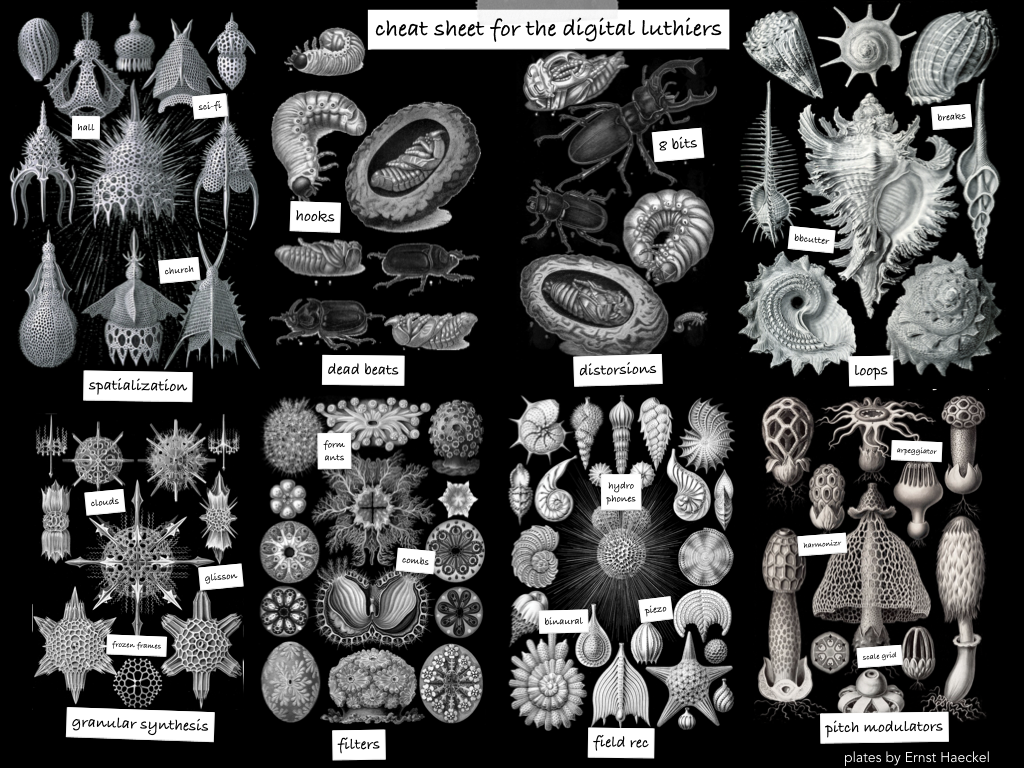
\includegraphics[width=\textwidth]{gfx/02_ephemeral/Bestiaire.png}
	\caption{Entomologie musicale}
	\label{fig:ephemeral:entomologie}
\end{figure}

\subsection{Pratique modulaire de la stabilité}

While a DMI can be an unstable assemblage, its individual components may provide more stable grips. For example, if the performance is based on a written score, the instrumentalist can learn the sequence of appropriate gestures necessary for its realisation\footnote{A interesting and critical example is the piece Aphasia by Mark Applebaum (https://youtu.be/wWt1qh67EnA), where the performance relies on gestures and a soundtrack which are totally notated, yet to be performed.}, such as a pilot in a cockpit \cite{vertegaal_towards_1996}.\\
\indent As far as the behaviour of the DMI is concerned, one can partly transfer one's knowledge of other DMIs to a new instance one is trying to learn. For example, the integration of an FM synthesis into a DMI can help a person familiar with this type of synthesis to navigate its timbre space (bells, siren, brassy, wiggly, etc.), independently of the control interface plugged onto it, relying on their own knowledge and representation of FM synthesis parameter space. The timbre space of various audio syntheses can also be remapped on a common and more stable perceptive space (e.g. pitch, loudness, brilliance, etc.) that abstracts control from their differing parameter spaces, such as presented in \cite{wessel_timbre_1979}, \cite{arfib_strategies_2002}, \cite{schwarz_sound_2012} or \cite{tubb_divergent_2014}.\\
\indent Likewise, an expertise can be acquired on a gestural interface, which calls for specific gestures and moves\footnote{For instance, consider the “launchpad” scene, characterized by the publication of battle-videos of rhythmic virtuosity.}; this expertise relies on an embodied spatial memory that—to some extent— remains partly independent from the audio syntheses or effects controlled with the interface. The behavioural stability of the instrument can also be of virtual nature, for example when using dynamic intermediate models \cite{goudard_dynamic_2011}, which can act as a stable reference taking place between various changing syntheses and interfaces.\\
\indent Overall, this transposed and “modular” knowledge can only provide broad outlines of what is necessary for the subtle practice of an instrument. The devil's is obviously to be found in the details.

\subsection{Les DMI comme vaisseau pour la mémoire}
\label{sec:ephemeral:vessels}
DMIs are heterogeneous vessels loaded with memories of our performing, composing or instrument-making experiences. The sounds that we collect, the synthesis algorithms that we develop (or download), the parameters that we adjust, the kitchen recipes and mapping functions that we carefully craft, all contribute to the evolution of a personal repertoire where ephemeral instances crystallize. Magnusson proposed the term epistemic tool to describe a musical instrument as \iquote{a designed tool with such a high degree of symbolic relevance that it becomes a system of knowledge and thinking in its own terms} \cite{magnusson_epistemic_2009}.\\
\indent Thus, DMIs tend to be evolving assemblages of these stored memories and often involve activities that are not generally associated with instrumental practice, such as file management, bookmarking online resources or organizing sound banks, in order to be able to convene these resources as quickly as possible during the performance.\\
\indent It is remarkable that the possibilities of duplication and dissemination offered by digital media and the Internet have not led to the standardisation of instrumentariums; digital musical instruments are often very personal and singular.

\section{Conclusion}

This article has presented how the ephemerality of DMIs should not only be considered as a problem, but as an intrinsic modality of their ontology. Rather than opposing longevity, it actually informs the technical design of the environments conducive to their development and sustainability.\\
\indent Ephemerality of the tools does not prevent great music to be produced, nor great musical performances to happen. On the contrary, it can both help to adapt musical assemblages to contexts that are in essence ephemeral and to challenge human's ability to respond to a fleeting, untamed musical setup. In the end, great musical works seem to find their way, sustained by the care and the work of those who recognize these works as master pieces. These works may stand the test of time being dispersed, distributed, transformed, recomposed, reinterpreted or even renamed, by all those who will attach importance to them. This loving care probably belongs to the part of our memory that we cannot outsource in a tool and that redefines tradition and preservation outside the technological frame.\\
\indent In the sand that was evoked by Michel Chion, we could see another interesting metaphor for digital musical instruments, as sand in a previous life was a rock that got atomized, fragmented into tiny bits. The same thing seem to have happened to musical instruments, that have been atomized into tiny modules. We can play with sand as a fluid material, or givin it a shape, or adding cement and make something more concrete.
\indent If digital technologies reach maturity one day, we may be able to rely on stable and sustainable instruments. In this case, following Garsault's premonition, it should not be forgotten to classify all the ephemeral instruments that preceded them in the category of \iquote{instruments out of use, but that could come back}.


\section{extra material}

Thor Magnusson in Sonic Writing (p12) : Anyone who plays a musical instrument will be familiar with the special moment when a new instrument is picked and its ergodynamics studied through play. (footnote : we often change our instruments during performance : we retune string instruments, change effect settings in electronics, and the \textit{whole point} of live coding is to create and redefine the instrument during play). This experience of ergodynamics recognises that an instrument is an object that never rests, or enter a period of stasis: that every time we pick it up there are new things to discover, new patterns our fingers know, because we have changed, the instrument has changed, and so has the whole world itself — the general performance context.

Risset dans \cite{genevois_les_1999} : ``La disponibilité `'d'accès'' gestuels tout à fait différents de accès instrumentaux risque de rester lettre morte, dans la mesure où il est improbable que des interprètes réalisent l'investissement considérable que représente l'apprenttissage d'un instrument complètement nouveaux s'ils n'ont pas l'assurance que cet instrument va durer et qu'un répertoire va se développer pour lui''

